\chapter{Wazuh}
\section{Entstehung}
Wazuh ist aus dem Open-Source Projekt \href{https://github.com/ossec}{ossec}\footnote{Link: https://github.com/ossec} entstanden.
Wazuh ist wie ossec komplett Open-Source und kostenlos verfügbar.

\section{Aufbau}
Wazuh basiert auf dem \acrfull{elk} Stack. 
Es ist ein Plugin, welches in den \acrshort{elk} Stack integriert werden kann und mithilfe von Agents auf den Computern Logdateien sammelt.

\begin{figure}[H]
    \centering
    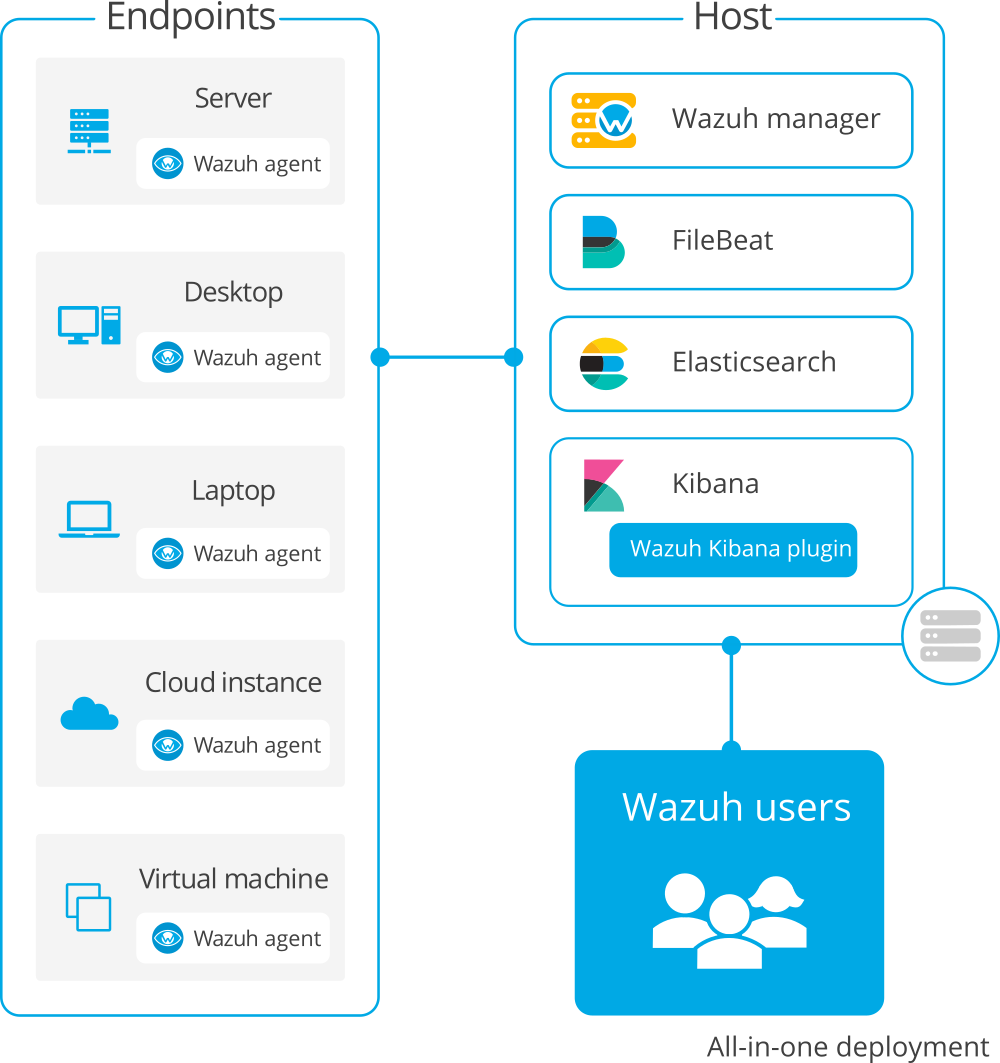
\includegraphics[width=\linewidth]{../img/aufbau-wazuh.png}
    \caption[Übersicht Wazuh]{Übersicht Wazuh\footnotemark}
\end{figure}
\footnotetext{Zugriff: 24.04.2022 \cite{wazuh-documentation}}

\subsection{Wazuh Manager}
Der Wazuh Manager wird auf einem Linux Server installiert.
Der Wazuh Manager beinhaltet den kompletten \acrshort{elk} Stack und das Wazuh Plugin. 

\subsubsection{ossec.conf}
In der ossec.conf Datei sind alle Konfigurationen vom Wazuh-Manager abgespeichert.

\subsection{Wazuh Agent}
Die Wazuh Agent werden auf den Computern installiert.
Es wird eine breite Sparte an Betriebssystemen unterstützt. Darunter viele Linux Systeme, Windows und MacOS.\\

Der Wazuh Agent leitet alle Logdateien, die in der agent.conf definiert sind, weiter an den Wazuh Manager.
Zusätzlich überwacht der Wazuh Agent auch alle Systemdatei- und Registryänderungen und leitet diese an den Wazuh Manager weiter. 

\subsection{Ablauf}
Die Agents senden die Logs an den Wazuh Manager oder der Wazuh Manager holt die Logs mit rsyslog von den Systemen. 
Danach werden die Logs mit einem Decoder strukturiert und die Regeln werden auf die Logs angewendet.
Wenn eine Regel zutrifft, wird ein Alert generiert und angezeigt.
Wenn keine Regel zutrifft, wird das Log verworfen.
In der ossec.conf kann eingestellt werden, dass auch die Logs abgespeichert werden, die auf keine Regel zutreffen.
Dabei sammeln sich jedoch grosse Datenmengen an und dies ist nur für Debugging empfohlen.

\begin{figure}[H]
    \centering
    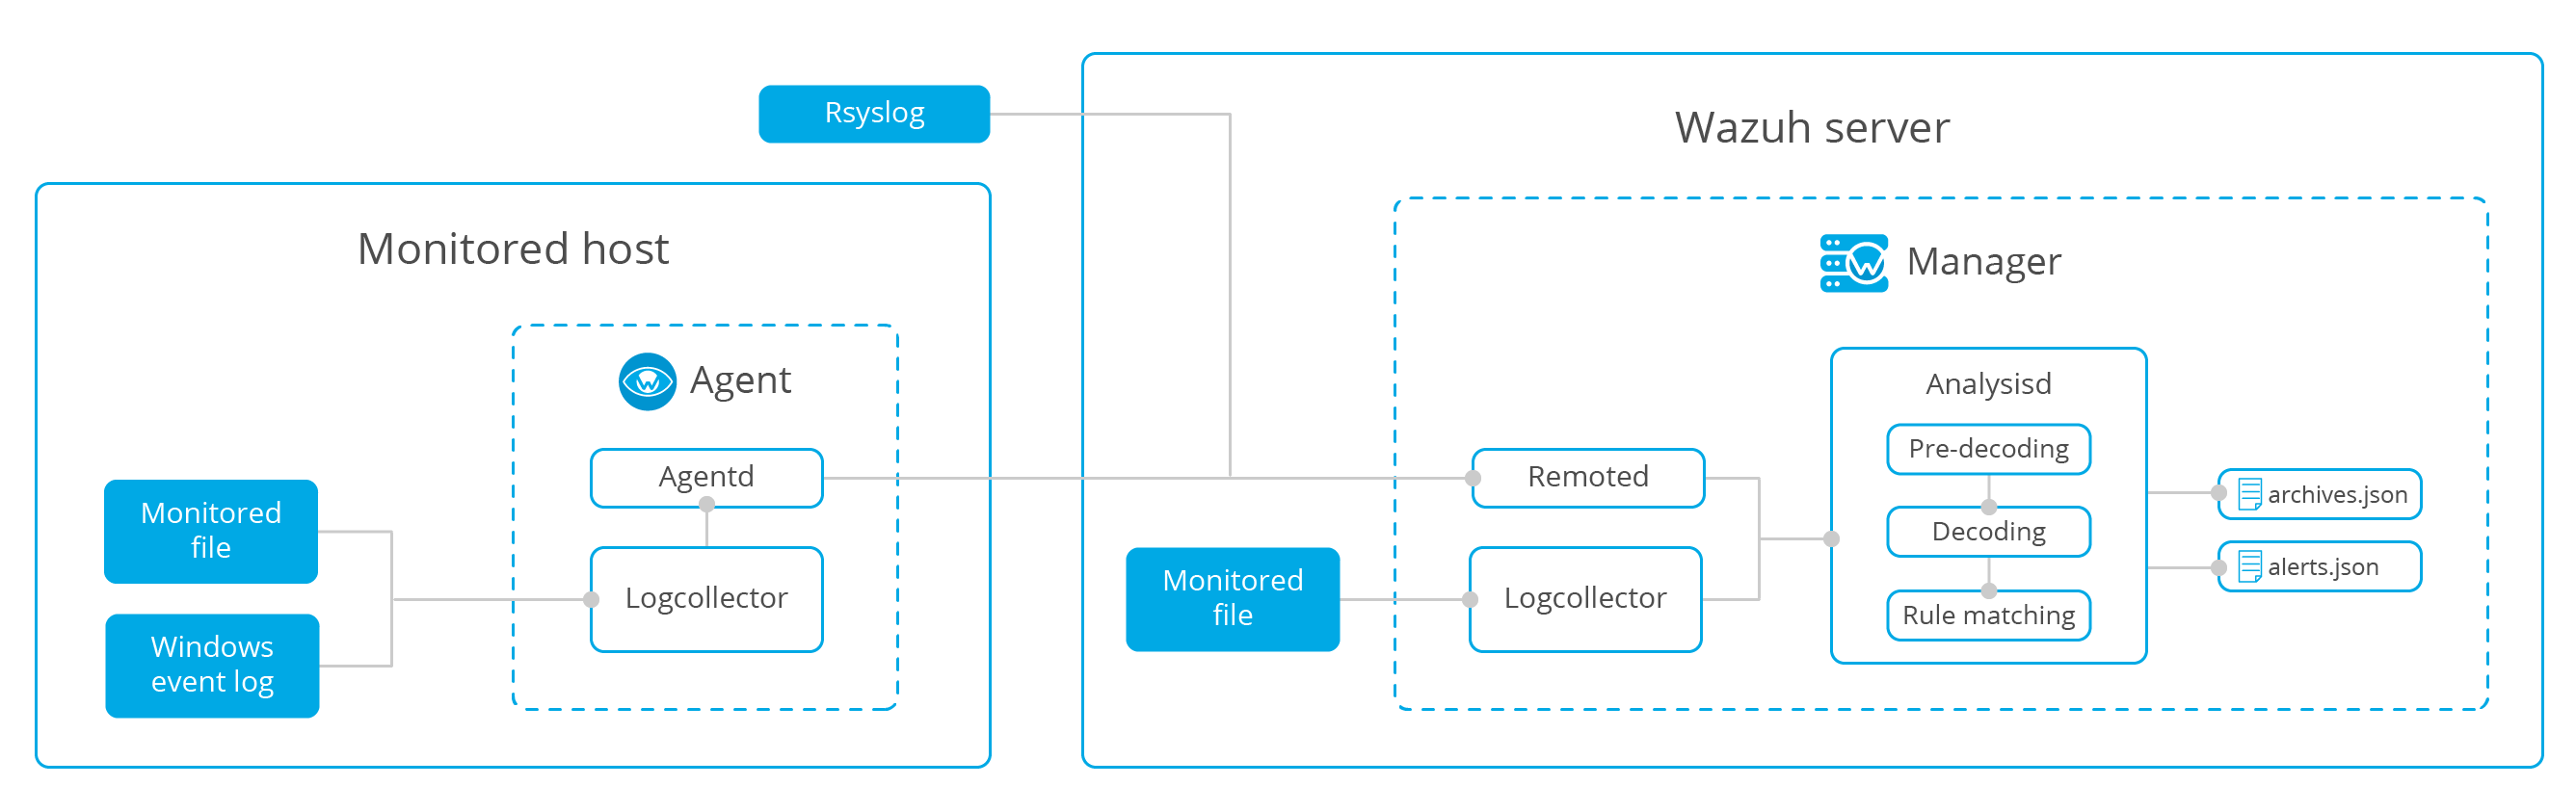
\includegraphics[width=\linewidth]{../img/wazuh-ablauf.png}
    \caption[Wazuh Ablauf]{Wazuh Ablauf\footnotemark}
\end{figure}
\footnotetext{Zugriff: 24.04.2022 \cite{wazuh-documentation}}

\section{Rules}
\subsection{Alert Level}
Es gibt Alert Levels von 0 bis 16. 
Diese bedeuten jedoch nicht wie schwerwiegen ein Ereignis ist, sondern jedes Level hat eine Beduetung.
Die wichtigsten Level sind folgende:
\begin{itemize}
    \item \textbf{Level 3} sind Alerts, welche Authorisiert sind und tendenziell nicht gefährlich.
    \item \textbf{Level 12} sind Alerts, welche eine Anomalie darstellen und potentiell gefährlich sind.
\end{itemize}

Alle Alert Level findet man in der \href{https://documentation.wazuh.com/current/user-manual/ruleset/rules-classification.html}{Wazuh Dokumentation}\footnote{Link: https://documentation.wazuh.com/current/user-manual/ruleset/rules-classification.html}.

\section{Decoders}
Da Logs in allen möglichen Formen kommen, je nach Herkunft, braucht es Decoder.
Die Decoder bringen die eingehenden Logs in eine einheitliche Struktur, um die Regeln darauf anwenden zu können.
Es werden Decoder für einige bekannten Logformate angeboten, wie zum Beispiel für den Windows Event Manager oder Cisco IOS Logs.


\section{Groups}
Die Gruppen werden verwendet, um ähnliche Geräte zu gruppieren.
Für jede Gruppe kann man eine agent.conf einrichten, in welcher eingetragen wird welche Logdateien von diesen Systemen verarbeitet werden sollen. 

\subsubsection{agent.conf}
In der agent.conf kann definiert werden, welche Logdateien an den Wazuh Manager weitergeleitet werden. 
Eine Lokation wird mit <localfile> angegeben:
\begin{lstlisting}
<agent_config os="Windows">
	<localfile>
		<location>Microsoft-Windows-Sysmon/Operational</location>
		<log_format>eventchannel</log_format>
	</localfile>
</agent_config>
\end{lstlisting}
Weitere Informationen wie neue Orte mit Logdateien eingebunden werden können, findet man in der \href{https://documentation.wazuh.com/current/user-manual/reference/centralized-configuration.html?highlight=agent%20conf}{Wazuh Dokumentation}\footnote{Link: https://documentation.wazuh.com/current/user-manual/reference/centralized-configuration.html?highlight=agent\%20conf}